\chapter{Modified Booth Encoding Multiplier}
\label{chap2}


\section{MBE Multiplier Design}
In order to complete the set of comparisons among different multiplier's implementations,
a modified-Booth-encoding multiplier for unsigned data has been designed. In the folder $MBE\_multiplier$, three subfolders
have been created, $src$, $tb$ and $sim$.
In order to follow the specifications given by the assignment, partial products have been
generated without using any adders or subtracters, the adder plane has been implemented
relying on a Dadda tree and sign extension bits have been simplified as proposed in the
file $sign\_extension\_booth\_multiplier\_Stanford.pdf$. Once the simulation has been carried
out to check its correctness, the MBE multiplier has been exploited in the Stage2 of the
floating point multiplier, instead of the behavioural one "$*$".

\begin{figure}[H]
	\centering
	\includegraphics[width=\textwidth , height=10cm]{img/MBE_Mult.png} 
	\caption{Modified Booth encoding multiplier block diagram}
	\label{Modified Booth encoding multiplier block diagram} 
\end{figure}

As depicted in figure, the main blocks used in this design are:

\begin{itemize}
 
\item \emph{MBE\_recoder}: based on the input triplet coming from the operand $b$, it provides the correct partial product 
at the output, according to the table shown in Figure 2.2;

\item \emph{A\_gen}: it generates the values that will be fed to the $MBE_recoder$. It takes
$a$ on 32 bits as input and it provides four 33-bit outputs, $a$ (setting '0' as MSB), $2a$,
1's complement $a$ and 1's complement $2a$;

\item \emph{Sign\_Ext}: it selects the value for $S$ as indicated in the file
$sign\_extension\_booth\_multiplier\_Stanford.pdf$. If the partial product is negative, $S$ will be 
equal to '1' in order to add 1 to the toggled version of $a$ or $2a$ and generate the correct
2's complement value. If the partial product is positive, $S$ will be '0' in order to clear
the sign extension bits;

\item \emph{Dadda\_Tree}: it performs the addition on the 17 sign-extended partial products as
stated by the Dadda algorithm. Starting from the initial "Staircase" form, partial products have
been reorganized in a "V-shape" structure, where each column contains equally-weighted bits. Also $S$
bits have been properly assigned. Since 17 partial products are present, 6 reduction operations have to be performed before having the final 2 operands on which a behavioural
addition has been perfomed. At each level, the minimum number of HA and FA have been assigned
in order to reach the next level's maximum heigth. As described by comments in file "Dadda\_Tree.vhd", a three-dimensional array has been exploited to have 7 different "V-shape" matrices, each corresponding to a reduction level. For each of this levels, the Dadda Algorithm has been applied, until reaching the final two partial products;

\end{itemize}


\begin{figure}[H]
	\centering
	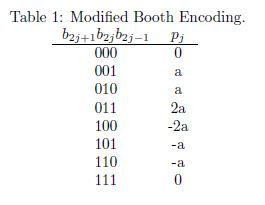
\includegraphics[width=8cm, height=6cm]{img/MBE.jpeg} 
	\caption{Recoding Table}
	\label{Recoding Table} 
\end{figure}


All these components have been used in the top entity "Dadda\_Multiplier", connected as depicted in
figure. As mentioned before, a behavioural adder "$+$" has been exploited in order to add the final
reduction level partial products.

\section{MBE Multiplier Simulation}

A simulation of the designed multiplier has been carried out using $tb\_Dadda\_Mul.vhd$ in subfolder $tb$. 
This testbench exploits a 32-bits LFSR generating the multiplier's inputs. The same values are given to a behavioural
unsigned multiplier in order to check the correctness. If the two outputs are equal, a "check signal" is equal to one.
The simulationn has been performed in the subfolder $sim$ using the script $compile.sh$ to compile the needed files.
It has been run for in order to verify the correct behaviour of the component and a $pdf$ file containing the resulting
waveforms has been saved.
\newline
\newline
Then, the a new file called $fpmul\_stage2\_struct\_MBE.vhd$ has been created starting from $fpmul\_stage2\_struct.vhd$
by replacing the behavioural multiplier with the MBE one. A new subfolder named $sim_MBE$ has been created in folder $sim$ and
the simulation has been run with the help of $compile.sh$. The resulting values have been checked and a $pdf$ file has been generated
with the obtained waveforms.

\section{MBE Multiplier Synthesis and Final Comparison}

Once the correctness has been verified, a subfolder called $syn\_MBE$ has been created in $syn$ and set as work environment for the
synthesis. It has been perfomed using a $tcl$ script and an iterative approach has been adopted in order to obtain the maximum frequency, as described in the previous paragraph. Moreover, an area report and a timing report have been produced in order to check the results concerning maximum frequency and area, which are summarized in Table along with all the others.



\begin{center}
    \begin{tabular}{ |c|c|c|c| } 
        \hline
            Name & $t_{min}$[$\si{\nano\second}$] & $f_{max}$[$\si{\mega\hertz}$] & area[$\si{\micro\meter}^{2}$]\\
            \hline
            syn\_first & 1.56 & 641.025641 & 4047.721967\\
            \hline
            syn\_CSA & 4.28 & 233.644859 & 3712.828004\\
            \hline
            syn\_PPARCH & 1.56 & 641.025641 & 4097.197964\\
            \hline
            syn\_modified & 0.87 & 1149.42528 & 5572.433932\\
            \hline
            syn\_modified\_ultra & 1.50 & 666.666666 & 4207.321944\\
            \hline
            syn\_MBE & 4.10 & 243.902439 & 6905.625925\\
        	\hline
    \end{tabular}
    \begin{center}
    	Tab 1: Comparisons Table.
    \end{center}
\end{center}


\subsection{Final Overall Comparisons}

Regarding the maximum frequency, the best result has been obtained with the synthesis using the command $optimize\_registers$, which applies a proper retiming. The same clock has been retrieved for the first synthesis and the one forcing a PPARCH implementation. This is due to the fact that a pparch architecture has been used by both of them, with the only difference in the radix used. In the first one a radix-4 has been adopted, while in the second a radix-8. The worst one in terms of timing is the CSA one, with $4.28\si{\nano\\second}$.
As shown in figure, the best one in terms of area occupation is the CSA, while the worst is the MBE implementation. As before, the first synthesis and the PPARCH one are very similar, with the latter a little bit greater than the first. As regards the $compile\_ultra$ results, it has a lower area occupation than the $optimize\_registers$ version. However, it also shows a greater clock period leading to a lower maximum frequency.